\chapter{Funciones y continuidad}
\label{ch:funciones}

En ingeniería es habitual describir una magnitud a partir de otra: la longitud de una barra cambia con la temperatura, la concentración de un reactivo evoluciona con el tiempo, la tensión de una red varía periódicamente y la potencia producida por una máquina depende de sus condiciones de funcionamiento. El lenguaje matemático que permite expresar estas dependencias es el de las funciones. En este capítulo estudiaremos las funciones reales de variable real, sus principales familias, el concepto de límite y la continuidad. Estos conceptos constituyen, además, la base sobre la que se construyen el cálculo diferencial y el cálculo integral.

\section{Funciones reales de variable real}
\label{sec:funciones-reales}

\subsection{Concepto de función, dominio, recorrido y gráfica}

Una variable es una cantidad que puede tomar distintos valores. Cuando los valores de una variable están determinados por los de otra, aparece de forma natural el concepto de función.

\begin{example}
El área de una sección circular depende de su radio. Si el radio es $r>0$, entonces
\[
A(r)=\pi r^2.
\]
En este modelo, $r$ es la variable independiente y $A$ la variable dependiente.
\end{example}

\begin{definition}[Función real de variable real]
Sean $D\subseteq\R$ y $f$ una regla que asigna a cada $x\in D$ un único número real $f(x)$. Diremos que
\[
f:D\longrightarrow\R
\]
es una \emph{función real de variable real}. El conjunto $D$ se denomina \emph{dominio} de $f$ y se denota $\operatorname{Dom}(f)$.
\end{definition}

El conjunto de valores que realmente toma la función se denomina \emph{recorrido} o \emph{imagen}:
\[
\operatorname{Im}(f)=\{f(x):x\in\operatorname{Dom}(f)\}.
\]
La notación
\[
y=f(x)
\]
indica que $x$ es la variable independiente y que $y$ depende de $x$.

Una función puede describirse mediante una fórmula, una tabla, una gráfica o una regla verbal. En aplicaciones, estas representaciones se complementan. Una tabla de medidas experimentales puede sugerir una gráfica y, a partir de ella, un modelo algebraico aproximado.

\begin{example}[Curva de calibración]
Un sensor de temperatura proporciona, dentro de su intervalo de trabajo, una tensión aproximadamente lineal
\[
V(T)=0.010T+0.50,
\]
donde $T$ se mide en grados Celsius y $V$ en voltios. La fórmula permite calcular la salida del sensor para cualquier temperatura admisible. Por ejemplo,
\[
V(80)=1.30\ \mathrm{V}.
\]
Si el fabricante especifica que el modelo es válido para $-20\leq T\leq150$, el dominio físico del modelo es $[-20,150]$, aunque la expresión algebraica $0.010T+0.50$ esté definida para todo $T\in\R$.
\end{example}

Esta distinción entre \emph{dominio matemático} y \emph{dominio de validez de un modelo} será importante a lo largo del curso.

\begin{definition}[Gráfica de una función]
La gráfica de una función $f:D\to\R$ es el conjunto
\[
G_f=\{(x,f(x)):x\in D\}\subseteq\R^2.
\]
\end{definition}

Una curva del plano representa una función de $x$ si toda recta vertical corta a la curva, como máximo, en un punto. Esta observación se conoce como \emph{criterio de la recta vertical}.

En muchas ocasiones la fórmula de una función determina su dominio de forma implícita. Cuando no se indique otra cosa, entenderemos por dominio el mayor subconjunto de $\R$ para el que la expresión tiene sentido.

Las restricciones más frecuentes son:
\begin{itemize}
\item un denominador no puede anularse;
\item el radicando de una raíz de índice par debe ser no negativo;
\item el argumento de un logaritmo debe ser estrictamente positivo.
\end{itemize}

\begin{example}
Determinar el dominio de
\[
f(x)=\frac{\sqrt{x+1}}{x-2}.
\]
Para que la raíz esté definida debe cumplirse $x+1\geq0$, es decir, $x\geq-1$. Además, el denominador exige $x\neq2$. Por tanto,
\[
\operatorname{Dom}(f)=[-1,2[\,\cup\,]2,+\infty[.
\]
\end{example}

\begin{solvedexercise}
Determinar el dominio de
\[
g(x)=\ln\!\left(\frac{x-1}{x+2}\right).
\]
\tcblower
\textbf{Resolución.}\par\smallskip
El argumento del logaritmo debe ser positivo:
\[
\frac{x-1}{x+2}>0.
\]
Los puntos que pueden cambiar el signo son $x=-2$ y $x=1$. El cociente es positivo en
\[
]-\infty,-2[\,\cup\,]1,+\infty[.
\]
Por tanto,
\[
\operatorname{Dom}(g)=]-\infty,-2[\,\cup\,]1,+\infty[.
\]
\end{solvedexercise}

Además del dominio y del recorrido, algunas propiedades globales proporcionan información cualitativa muy útil.

\begin{definition}[Paridad]
Sea $f:D\to\R$ y supongamos que $x\in D\Rightarrow -x\in D$.
\begin{itemize}
\item $f$ es \emph{par} si $f(-x)=f(x)$ para todo $x\in D$.
\item $f$ es \emph{impar} si $f(-x)=-f(x)$ para todo $x\in D$.
\end{itemize}
\end{definition}

La gráfica de una función par es simétrica respecto del eje vertical, mientras que la de una función impar es simétrica respecto del origen.

\begin{definition}[Periodicidad]
Una función $f$ es \emph{periódica} si existe $T>0$ tal que
\[
f(x+T)=f(x)
\]
siempre que $x$ y $x+T$ pertenezcan al dominio. Un valor $T$ con esta propiedad se denomina período. Cuando existe un período positivo mínimo, éste se denomina \emph{período fundamental}.
\end{definition}

La periodicidad aparece de forma natural en fenómenos oscilatorios. Por ejemplo, una tensión sinusoidal ideal puede escribirse como
\[
v(t)=V_0\sin(\omega t+\varphi),
\]
y tiene período
\[
T=\frac{2\pi}{\omega}.
\]

\begin{definition}[Monotonía]
Sea $I$ un intervalo. Una función $f$ es \emph{creciente} en $I$ si
\[
x_1<x_2\Longrightarrow f(x_1)\leq f(x_2),
\]
y \emph{estrictamente creciente} si la desigualdad es estricta. Análogamente, $f$ es \emph{decreciente} en $I$ si
\[
x_1<x_2\Longrightarrow f(x_1)\geq f(x_2).
\]
\end{definition}

\begin{definition}[Acotación]
Sea $A\subseteq\operatorname{Dom}(f)$.
\begin{itemize}
\item $f$ está acotada superiormente en $A$ si existe $M\in\R$ tal que $f(x)\leq M$ para todo $x\in A$.
\item $f$ está acotada inferiormente en $A$ si existe $m\in\R$ tal que $f(x)\geq m$ para todo $x\in A$.
\item $f$ está acotada en $A$ si está acotada superior e inferiormente.
\end{itemize}
\end{definition}

Por ejemplo, $\sin x$ y $\cos x$ están acotadas entre $-1$ y $1$, una propiedad que tiene interpretación inmediata cuando representan magnitudes sinusoidales normalizadas.

\subsection{Funciones elementales}

Las funciones que aparecerán con mayor frecuencia pueden construirse a partir de unas pocas familias elementales.

\paragraph{Funciones polinómicas y racionales.}
Una función polinómica tiene la forma
\[
p(x)=a_nx^n+a_{n-1}x^{n-1}+\cdots+a_1x+a_0,
\qquad a_n\neq0,
\]
y está definida para todo $x\in\R$. Una función racional es un cociente
\[
r(x)=\frac{p(x)}{q(x)},
\]
donde $p$ y $q$ son polinomios y
\[
\operatorname{Dom}(r)=\{x\in\R:q(x)\neq0\}.
\]

Las funciones lineales y cuadráticas son casos particulares de funciones polinómicas. Una relación lineal
\[
y=mx+b
\]
representa una dependencia con tasa de variación constante. Una función cuadrática
\[
y=ax^2+bx+c,
\qquad a\neq0,
\]
tiene como gráfica una parábola.

\begin{example}[Deformación térmica]
En un intervalo moderado de temperaturas, la longitud de una barra puede modelarse por
\[
L(T)=L_0\bigl(1+\alpha(T-T_0)\bigr).
\]
Como función de $T$, se trata de una función lineal. El parámetro $\alpha$ mide cuánto cambia proporcionalmente la longitud por unidad de temperatura. El modelo no pretende describir temperaturas arbitrarias: su dominio físico es el intervalo en el que la aproximación lineal sea válida.
\end{example}

\paragraph{Funciones potenciales y radicales.}
Una función potencial tiene la forma
\[
f(x)=x^r,
\]
con exponente real $r$, en el dominio en el que la potencia esté definida como número real. Son especialmente frecuentes las potencias enteras y las raíces.

Por ejemplo,
\[
f(x)=\sqrt{x}
\]
tiene dominio $[0,+\infty[$ y recorrido $[0,+\infty[$, mientras que
\[
g(x)=\frac{1}{x}
\]
tiene dominio $\R\setminus\{0\}$.

\paragraph{Funciones exponenciales y logarítmicas.}
Sea $a>0$, $a\neq1$. La función exponencial de base $a$ es
\[
f(x)=a^x.
\]
Su dominio es $\R$, su recorrido es $]0,+\infty[$ y nunca se anula. Si $a>1$ es estrictamente creciente y si $0<a<1$ es estrictamente decreciente.

La base exponencial más importante es
\[
e=2.718281828\ldots,
\]
y escribiremos
\[
\exp(x)=e^x.
\]

La función logarítmica de base $a$ se define como la inversa de la exponencial:
\[
\log_a(x)=y\Longleftrightarrow a^y=x.
\]
Su dominio es $]0,+\infty[$ y su recorrido es $\R$. Para la base $e$ utilizaremos el logaritmo natural
\[
\ln x=\log_e x.
\]
Se verifican, para $x,y>0$,
\[
\ln(xy)=\ln x+\ln y,
\qquad
\ln\left(\frac{x}{y}\right)=\ln x-\ln y,
\qquad
\ln(x^r)=r\ln x.
\]

\begin{example}[Decaimiento de una concentración]
En un modelo de cinética de primer orden, la concentración de un reactivo puede escribirse como
\[
C(t)=C_0e^{-kt},\qquad t\geq0,
\]
donde $C_0>0$ es la concentración inicial y $k>0$ una constante característica del proceso. La función es positiva y decreciente, y satisface
\[
\frac{C(t)}{C_0}=e^{-kt}.
\]
Si se quiere conocer el instante en que la concentración se reduce a la mitad, se resuelve
\[
e^{-kt}=\frac12,
\]
de donde
\[
t=\frac{\ln2}{k}.
\]
El logaritmo aparece, por tanto, de forma natural al despejar una variable situada en un exponente.
\end{example}

\paragraph{Funciones trigonométricas.}
Las funciones seno y coseno tienen dominio $\R$, recorrido $[-1,1]$ y período fundamental $2\pi$:
\[
\sin(x+2\pi)=\sin x,
\qquad
\cos(x+2\pi)=\cos x.
\]
Además,
\[
\sin^2x+\cos^2x=1.
\]
La tangente se define por
\[
\tan x=\frac{\sin x}{\cos x}
\]
y su dominio es
\[
\R\setminus\left\{\frac{\pi}{2}+k\pi:k\in\Z\right\}.
\]

Los argumentos de las funciones trigonométricas se medirán en radianes. Recordemos que
\[
\pi\ \text{radianes}=180^\circ.
\]

\begin{example}[Movimiento armónico]
La posición de una masa sometida a una oscilación ideal puede modelarse por
\[
x(t)=0.04\cos(10t)\quad \text{m}.
\]
La amplitud es $0.04\,\mathrm{m}$ y el período de la oscilación es
\[
T=\frac{2\pi}{10}=\frac{\pi}{5}\ \mathrm{s}.
\]
La propia forma de la función permite leer propiedades físicas sin realizar ningún cálculo diferencial.
\end{example}

Las funciones trigonométricas inversas se obtienen restringiendo adecuadamente los dominios. Utilizaremos
\[
\arcsin:[-1,1]\to\left[-\frac\pi2,\frac\pi2\right],
\]
\[
\arccos:[-1,1]\to[0,\pi],
\qquad
\arctan:\R\to\left]-\frac\pi2,\frac\pi2\right[.
\]

En la Figura~\ref{fig:elementales-t2} se muestran algunas funciones elementales que servirán de referencia durante el curso.

\begin{figure}[H]
\centering
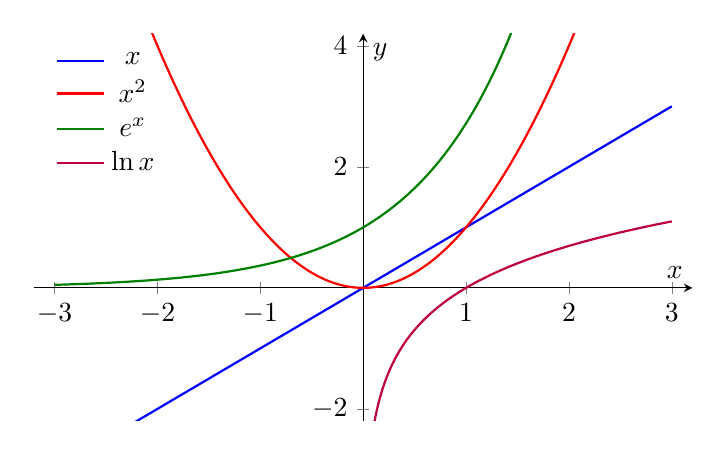
\begin{tikzpicture}
\begin{axis}[
  width=.82\textwidth,height=6.5cm,
  axis lines=middle,
  xmin=-3.2,xmax=3.2,ymin=-2.2,ymax=4.2,
  xlabel={$x$},ylabel={$y$},
  samples=160,
  legend style={at={(0.02,0.98)},anchor=north west,draw=none,fill=none},
  domain=-3:3
]
\addplot[thick,blue] {x};
\addlegendentry{$x$}
\addplot[thick,red] {x^2};
\addlegendentry{$x^2$}
\addplot[thick,green!50!black] {exp(x)};
\addlegendentry{$e^x$}
\addplot[thick,purple,domain=0.06:3] {ln(x)};
\addlegendentry{$\ln x$}
\end{axis}
\end{tikzpicture}
\caption{Algunas funciones elementales.}
\label{fig:elementales-t2}
\end{figure}

\paragraph{Transformaciones de gráficas.}
A partir de la gráfica de una función $f$ pueden obtenerse otras mediante transformaciones sencillas. Si $c>0$:
\[
f(x)+c
\]
desplaza la gráfica $c$ unidades hacia arriba,
\[
f(x-c)
\]
la desplaza $c$ unidades hacia la derecha,
\[
-f(x)
\]
la refleja respecto del eje horizontal y
\[
f(-x)
\]
la refleja respecto del eje vertical.

Estas reglas son útiles para reconocer gráficas sin construir largas tablas de valores.

\subsection{Composición y función inversa}

Si $f$ y $g$ son funciones reales, podemos definir, en los puntos donde tenga sentido,
\[
(f+g)(x)=f(x)+g(x),\qquad
(fg)(x)=f(x)g(x),
\]
\[
\left(\frac fg\right)(x)=\frac{f(x)}{g(x)},\qquad g(x)\neq0.
\]
El dominio de la nueva función se obtiene intersectando los dominios de las funciones que intervienen y añadiendo las restricciones que correspondan.

La composición formaliza dependencias encadenadas.

\begin{definition}[Composición]
Sean $g:D_g\to\R$ y $f:D_f\to\R$. La función compuesta $f\circ g$ se define por
\[
(f\circ g)(x)=f(g(x))
\]
para aquellos $x\in D_g$ tales que $g(x)\in D_f$.
\end{definition}

\begin{example}[Cadena de conversión]
Un transmisor proporciona una tensión $V$ en función de una presión $p$ mediante
\[
V(p)=0.02p+1,
\]
y un sistema de adquisición convierte esa tensión en una lectura digital
\[
N(V)=1000V.
\]
La lectura en función de la presión es la composición
\[
(N\circ V)(p)=1000(0.02p+1)=20p+1000.
\]
El modelo completo se obtiene componiendo los modelos de cada etapa.
\end{example}

En general,
\[
f\circ g\neq g\circ f.
\]

\begin{definition}[Función inyectiva]
Una función $f:D\to\R$ es \emph{inyectiva} si
\[
f(x_1)=f(x_2)\Longrightarrow x_1=x_2.
\]
Equivalentemente, valores distintos de la variable independiente producen valores distintos de la función.
\end{definition}

Si $f$ es inyectiva, puede definirse una función inversa sobre su imagen.

\begin{definition}[Función inversa]
Sea $f:D\to\operatorname{Im}(f)$ una función inyectiva. Su función inversa
\[
f^{-1}:\operatorname{Im}(f)\to D
\]
se caracteriza por
\[
f^{-1}(f(x))=x,
\qquad
f(f^{-1}(y))=y.
\]
\end{definition}

No debe confundirse $f^{-1}(x)$ con $1/f(x)$. Las gráficas de $f$ y $f^{-1}$ son simétricas respecto de la recta $y=x$.

\begin{proposition}
Toda función estrictamente monótona en un intervalo es inyectiva en ese intervalo y, por tanto, admite función inversa sobre su imagen.
\end{proposition}

Por ejemplo, $e^x$ y $\ln x$ son funciones inversas entre sí. La función $x^2$ no es inyectiva en $\R$, pero sí lo es al restringirla a $[0,+\infty[$; en ese intervalo su inversa es $\sqrt{x}$.

\paragraph{Comprobación con Mathematica.}
Para representar una función en un intervalo utilizaremos fundamentalmente \texttt{Plot}. Por ejemplo,
\begin{mathematicacode}
Plot[{Exp[x], Log[x]}, {x, 0.1, 2}]
\end{mathematicacode}
La representación gráfica es una herramienta de exploración y comprobación; no sustituye al análisis del dominio ni a la justificación de las propiedades de la función.

\section{Límites}
\label{sec:limites}

El concepto de límite permite describir el comportamiento de una función cuando la variable independiente se aproxima a un punto, aunque la función no esté definida en ese punto. Esta idea hará posible definir en el capítulo siguiente la velocidad instantánea, la pendiente de una curva y, en general, la derivada.

\subsection{Límite en un punto y límites laterales}

De forma intuitiva, decir que $f(x)$ se aproxima a $L$ cuando $x$ se aproxima a $a$ significa que podemos hacer $f(x)$ tan próxima a $L$ como queramos tomando $x$ suficientemente próxima a $a$, sin exigir $x=a$.

\begin{definition}[Límite de una función]
Sea $f:D\subseteq\R\to\R$ y sea $a$ un punto al que pueden aproximarse puntos de $D$ distintos de $a$. Diremos que
\[
\lim_{x\to a}f(x)=L
\]
si para todo $\varepsilon>0$ existe $\delta>0$ tal que
\[
x\in D,\quad 0<|x-a|<\delta
\quad\Longrightarrow\quad
|f(x)-L|<\varepsilon.
\]
\end{definition}

La definición no exige que $f(a)$ exista. El límite describe lo que sucede \emph{alrededor} de $a$, no necesariamente en $a$.

\begin{example}
Sea
\[
f(x)=\frac{x^2-1}{x-1},\qquad x\neq1.
\]
Como
\[
f(x)=x+1\qquad (x\neq1),
\]
cuando $x$ se aproxima a $1$, $f(x)$ se aproxima a $2$. Por tanto,
\[
\lim_{x\to1}\frac{x^2-1}{x-1}=2,
\]
aunque la expresión original no esté definida en $x=1$.
\end{example}

En la recta real podemos aproximarnos a un punto desde valores menores o mayores.

\begin{definition}[Límites laterales]
Diremos que
\[
\lim_{x\to a^-}f(x)=L
\]
si $f(x)$ se aproxima a $L$ cuando $x$ se aproxima a $a$ con $x<a$. Análogamente,
\[
\lim_{x\to a^+}f(x)=L
\]
se refiere a la aproximación con $x>a$.
\end{definition}

\begin{theorem}
Existe $\displaystyle\lim_{x\to a}f(x)=L$ si y sólo si existen los dos límites laterales y
\[
\lim_{x\to a^-}f(x)=\lim_{x\to a^+}f(x)=L.
\]
\end{theorem}

\begin{example}
Consideremos
\[
f(x)=
\begin{cases}
2x+1, & x<1,\\
x^2+2, & x\geq1.
\end{cases}
\]
Entonces
\[
\lim_{x\to1^-}f(x)=3,
\qquad
\lim_{x\to1^+}f(x)=3.
\]
Por tanto,
\[
\lim_{x\to1}f(x)=3.
\]
En este caso, además, $f(1)=3$; más adelante veremos que la función es continua en $x=1$.
\end{example}

Los límites se comportan bien respecto de las operaciones algebraicas.

\begin{proposition}[Álgebra de límites]
Si
\[
\lim_{x\to a}f(x)=A,
\qquad
\lim_{x\to a}g(x)=B,
\]
entonces, siempre que las expresiones estén definidas,
\begin{align*}
\lim_{x\to a}(f(x)\pm g(x))&=A\pm B,\\
\lim_{x\to a}f(x)g(x)&=AB,\\
\lim_{x\to a}\frac{f(x)}{g(x)}&=\frac AB,\qquad B\neq0.
\end{align*}
Además, para las potencias y composiciones de funciones continuas pueden aplicarse las reglas habituales de sustitución.
\end{proposition}

En particular, si una función elemental es continua en $a$, su límite en $a$ se obtiene sustituyendo $x=a$.

\subsection{Límites infinitos, límites en el infinito y asíntotas}

En ocasiones los valores de una función crecen sin cota cuando $x$ se aproxima a un punto. Utilizaremos entonces la notación de límite infinito.

\begin{definition}[Límite infinito]
Escribiremos
\[
\lim_{x\to a}f(x)=+\infty
\]
si para todo $M>0$ existe $\delta>0$ tal que
\[
x\in D,\quad 0<|x-a|<\delta\Longrightarrow f(x)>M.
\]
La definición de límite $-\infty$ es análoga.
\end{definition}

El símbolo $+\infty$ no representa un número real. La notación anterior expresa un comportamiento de la función.

Si al menos uno de los límites laterales en $a$ es infinito, la recta
\[
x=a
\]
se denomina \emph{asíntota vertical} de la gráfica.

\begin{example}
Para
\[
f(x)=\frac{1}{x-2}
\]
se tiene
\[
\lim_{x\to2^-}f(x)=-\infty,
\qquad
\lim_{x\to2^+}f(x)=+\infty.
\]
Por tanto, $x=2$ es una asíntota vertical.
\end{example}

También podemos estudiar el comportamiento para valores de $x$ arbitrariamente grandes en valor absoluto.

\begin{definition}[Límite en el infinito]
Supongamos que $D$ no está acotado superiormente. Diremos que
\[
\lim_{x\to+\infty}f(x)=L
\]
si para todo $\varepsilon>0$ existe $M>0$ tal que
\[
x\in D,\quad x>M\Longrightarrow |f(x)-L|<\varepsilon.
\]
Análogamente se define el límite cuando $x\to-\infty$ si $D$ no está acotado inferiormente.
\end{definition}

Si
\[
\lim_{x\to+\infty}f(x)=L
\quad\text{o}\quad
\lim_{x\to-\infty}f(x)=L,
\]
la recta $y=L$ es una \emph{asíntota horizontal} por el lado correspondiente.

\begin{example}[Respuesta estacionaria]
Consideremos
\[
T(t)=T_a+(T_0-T_a)e^{-kt},\qquad k>0,
\]
como modelo idealizado de la temperatura de un cuerpo que intercambia calor con un ambiente a temperatura $T_a$. Puesto que
\[
\lim_{t\to+\infty}e^{-kt}=0,
\]
se obtiene
\[
\lim_{t\to+\infty}T(t)=T_a.
\]
La recta $T=T_a$ es una asíntota horizontal del modelo y expresa matemáticamente que la temperatura se aproxima al equilibrio con el ambiente.
\end{example}

Una asíntota puede ser también oblicua.

\begin{definition}[Asíntota oblicua]
La recta $y=mx+n$, con $m\neq0$, es una asíntota oblicua de $f$ cuando $x\to+\infty$ si
\[
\lim_{x\to+\infty}\bigl(f(x)-(mx+n)\bigr)=0.
\]
Si existen los límites correspondientes, sus coeficientes pueden obtenerse mediante
\[
m=\lim_{x\to+\infty}\frac{f(x)}x,
\qquad
n=\lim_{x\to+\infty}\bigl(f(x)-mx\bigr).
\]
Se procede análogamente cuando $x\to-\infty$.
\end{definition}

\begin{example}
Sea
\[
f(x)=\frac{x^2-2x+4}{x-2}.
\]
Dividiendo polinomios,
\[
f(x)=x+\frac{4}{x-2}.
\]
Como
\[
\lim_{x\to\pm\infty}\frac{4}{x-2}=0,
\]
la recta
\[
y=x
\]
es una asíntota oblicua tanto cuando $x\to+\infty$ como cuando $x\to-\infty$. Además, $x=2$ es una asíntota vertical.
\end{example}

\subsection{Cálculo de límites e indeterminaciones}

Cuando la sustitución directa produce un valor real y todas las operaciones son válidas, el límite queda determinado inmediatamente. Sin embargo, ciertas expresiones no permiten decidir el resultado por sustitución. Las más habituales son
\[
\frac00,\qquad \frac{\infty}{\infty},\qquad
\infty-\infty,\qquad 0\cdot\infty,
\qquad 1^\infty,
\]
y también pueden aparecer $0^0$ o $\infty^0$. Se denominan \emph{formas indeterminadas}: dos expresiones distintas con la misma forma pueden tener límites diferentes.

No existe una única técnica para resolverlas. La transformación adecuada depende de la estructura de la expresión.

\paragraph{Factorización y simplificación.}
Cuando aparece $0/0$ en cocientes algebraicos, puede ser posible factorizar y cancelar un factor que sólo se anula en el punto al que tiende $x$.

\begin{example}
\[
\lim_{x\to1}\frac{x^3-x^2+x-1}{x-1}
=\lim_{x\to1}\frac{(x-1)(x^2+1)}{x-1}
=\lim_{x\to1}(x^2+1)=2.
\]
La cancelación es válida en el cálculo del límite porque se trabaja con $x\neq1$ suficientemente próximo a $1$.
\end{example}

\paragraph{Racionalización.}
Cuando intervienen raíces, multiplicar por la expresión conjugada puede eliminar la indeterminación.

\begin{example}
\[
\lim_{x\to0}\frac{\sqrt{1+x}-1}{x}
=\lim_{x\to0}
\frac{1}{\sqrt{1+x}+1}
=\frac12.
\]
\end{example}

\paragraph{Comparación de órdenes de crecimiento.}
Para $x\to+\infty$ resulta útil recordar que, para $a>1$ y $m,n\in\N$,
\[
a^x\gg x^n\gg (\ln x)^m,
\]
es decir, las exponenciales crecientes dominan a las potencias y éstas dominan a los logaritmos. Entre polinomios, el término de mayor grado determina el comportamiento en el infinito.

Por tanto, si
\[
r(x)=\frac{a_nx^n+\cdots+a_0}{b_mx^m+\cdots+b_0},
\qquad a_n b_m\neq0,
\]
entonces, cuando $x\to\pm\infty$, basta comparar $n$ y $m$ para determinar el comportamiento dominante. Si $n=m$, el límite es $a_n/b_m$; si $n<m$, el límite es $0$; y si $n>m$, el cociente no tiene límite finito en general.

\begin{example}
\[
\lim_{x\to+\infty}\frac{5x^2+3x-1}{-2x^2+7}
=-\frac52.
\]
Dividiendo numerador y denominador entre $x^2$ se obtiene directamente el cociente de los coeficientes principales.
\end{example}

\paragraph{La indeterminación $1^\infty$.}
El número $e$ puede caracterizarse mediante
\[
e=\lim_{n\to\infty}\left(1+\frac1n\right)^n.
\]
Más generalmente, si
\[
f(x)\to1,
\qquad
g(x)\to\pm\infty,
\]
y existe el límite indicado, entonces
\[
\lim_{x\to a}f(x)^{g(x)}
=
\exp\left(\lim_{x\to a}g(x)(f(x)-1)\right).
\]

\begin{example}
Calcular
\[
\lim_{x\to+\infty}\left(1+\frac{3}{x}\right)^x.
\]
Tomando
\[
f(x)=1+\frac3x,
\qquad g(x)=x,
\]
se tiene
\[
\lim_{x\to+\infty}g(x)(f(x)-1)
=\lim_{x\to+\infty}x\frac3x=3,
\]
y, por tanto,
\[
\lim_{x\to+\infty}\left(1+\frac3x\right)^x=e^3.
\]
\end{example}

Una herramienta especialmente útil en este tema es la equivalencia de infinitésimos.

\begin{definition}[Infinitésimo]
Una función $f$ es un infinitésimo cuando $x\to a$ si
\[
\lim_{x\to a}f(x)=0.
\]
\end{definition}

\begin{definition}[Infinitésimos equivalentes]
Sean $f$ y $g$ infinitésimos cuando $x\to a$. Diremos que son equivalentes, y escribiremos
\[
f(x)\sim g(x)\qquad(x\to a),
\]
si
\[
\lim_{x\to a}\frac{f(x)}{g(x)}=1.
\]
\end{definition}

Cuando $u\to0$, las equivalencias fundamentales que utilizaremos son
\[
\sin u\sim u,
\qquad
\tan u\sim u,
\qquad
\ln(1+u)\sim u,
\]
\[
e^u-1\sim u,
\qquad
1-\cos u\sim\frac{u^2}{2}.
\]
Más generalmente, para $a>0$,
\[
a^u-1\sim u\ln a.
\]

Estas equivalencias pueden sustituirse dentro de productos y cocientes en el cálculo de límites, pero no de forma indiscriminada dentro de sumas y diferencias.

\begin{solvedexercise}
Calcular
\[
\lim_{x\to0}\frac{\sin(3x)\,\ln(1+2x)}{x^2}.
\]
\tcblower
\textbf{Resolución.}\par\smallskip
Cuando $x\to0$,
\[
\sin(3x)\sim3x,
\qquad
\ln(1+2x)\sim2x.
\]
Por tanto,
\[
\frac{\sin(3x)\ln(1+2x)}{x^2}
\sim
\frac{(3x)(2x)}{x^2}=6,
\]
y
\[
\boxed{\displaystyle
\lim_{x\to0}\frac{\sin(3x)\ln(1+2x)}{x^2}=6.}
\]
\end{solvedexercise}

\begin{example}[Pequeñas oscilaciones]
En mecánica y electricidad aparecen aproximaciones de pequeño ángulo. Si $\theta$ se mide en radianes y $|\theta|$ es pequeño,
\[
\sin\theta\approx\theta.
\]
La justificación matemática local es precisamente
\[
\frac{\sin\theta}{\theta}\longrightarrow1
\qquad(\theta\to0).
\]
La aproximación no afirma que las dos funciones sean iguales; afirma que su error relativo se hace pequeño cerca de cero.
\end{example}

\paragraph{Comprobación con Mathematica.}
El comando básico para calcular límites será \texttt{Limit}. Por ejemplo,
\begin{mathematicacode}
Limit[Sin[3 x] Log[1 + 2 x]/x^2, x -> 0]
\end{mathematicacode}
y para límites en el infinito se utiliza \texttt{Infinity}:
\begin{mathematicacode}
Limit[(5 x^2 + 3 x - 1)/(-2 x^2 + 7), x -> Infinity]
\end{mathematicacode}
El cálculo con ordenador debe servir para verificar el resultado y explorar el comportamiento de la función, no para sustituir la identificación de la indeterminación y la elección de una técnica adecuada.

\section{Continuidad}
\label{sec:continuidad}

La continuidad formaliza una idea geométrica sencilla: una pequeña variación de la variable independiente produce una pequeña variación de la función. En modelos físicos, la continuidad suele ser una hipótesis razonable mientras no se atraviesen cambios de régimen, conmutaciones, impactos o transiciones de fase que introduzcan saltos u otras singularidades.

\subsection{Continuidad}

\begin{definition}[Continuidad]
Sea $f:D\subseteq\R\to\R$ y $a\in D$. Diremos que $f$ es \emph{continua en $a$} si
\[
\lim_{x\to a}f(x)=f(a).
\]
Equivalentemente, para todo $\varepsilon>0$ existe $\delta>0$ tal que
\[
x\in D,\quad |x-a|<\delta
\Longrightarrow
|f(x)-f(a)|<\varepsilon.
\]
\end{definition}

Para comprobar la continuidad en un punto interior del dominio pueden separarse tres condiciones:
\begin{enumerate}
\item $f(a)$ está definida;
\item existe $\displaystyle\lim_{x\to a}f(x)$;
\item $\displaystyle\lim_{x\to a}f(x)=f(a)$.
\end{enumerate}

\begin{definition}[Continuidad en un intervalo]
Una función es continua en un intervalo abierto si es continua en cada uno de sus puntos. En un intervalo cerrado $[a,b]$ se exige continuidad en $]a,b[$, continuidad por la derecha en $a$ y continuidad por la izquierda en $b$.
\end{definition}

Las funciones polinómicas son continuas en $\R$. Las racionales son continuas donde el denominador no se anula. Las funciones exponenciales, trigonométricas y las funciones potenciales son continuas en sus dominios; los logaritmos son continuos en $]0,+\infty[$.

\begin{proposition}[Operaciones con funciones continuas]
Si $f$ y $g$ son continuas en $a$, entonces también lo son
\[
f+g,\qquad f-g,\qquad fg,
\]
y
\[
\frac fg
\]
si $g(a)\neq0$. Además, si $g$ es continua en $a$ y $f$ es continua en $g(a)$, entonces $f\circ g$ es continua en $a$.
\end{proposition}

\begin{solvedexercise}
Determinar el valor de $k$ para que
\[
f(x)=
\begin{cases}
x^2, & x\leq1,\\
3x+k, & x>1
\end{cases}
\]
sea continua en $\R$.
\tcblower
\textbf{Resolución.}\par\smallskip
Cada expresión es continua en su intervalo. El único punto que debe estudiarse es $x=1$. Tenemos
\[
f(1)=1,
\qquad
\lim_{x\to1^-}f(x)=1,
\]
y
\[
\lim_{x\to1^+}f(x)=3+k.
\]
La continuidad exige
\[
3+k=1,
\]
de donde
\[
\boxed{k=-2.}
\]
\end{solvedexercise}

Las discontinuidades pueden clasificarse atendiendo al comportamiento de los límites.

\begin{itemize}
\item Una discontinuidad es \emph{evitable} si existe un límite finito en $a$ pero $f(a)$ no está definida o no coincide con ese límite. Puede eliminarse redefiniendo $f(a)$.
\item Hay una discontinuidad de \emph{salto} si existen límites laterales finitos pero son distintos.
\item Hay una discontinuidad \emph{infinita} si al menos uno de los límites laterales es infinito.
\end{itemize}

\begin{example}
La función
\[
f(x)=\frac{x^2-4}{x-2},\qquad x\neq2,
\]
presenta una discontinuidad evitable en $x=2$, pues
\[
\lim_{x\to2}f(x)=\lim_{x\to2}(x+2)=4.
\]
Definiendo $f(2)=4$ se obtiene una función continua en todo $\R$.
\end{example}

\subsection{Teoremas fundamentales de las funciones continuas}

La continuidad permite obtener conclusiones globales a partir de información local o de los valores en los extremos de un intervalo.

\begin{theorem}[Teorema del valor intermedio]
Sea $f:[a,b]\to\R$ continua. Si $k$ está comprendido entre $f(a)$ y $f(b)$, entonces existe $c\in[a,b]$ tal que
\[
f(c)=k.
\]
\end{theorem}

Una consecuencia fundamental es el Teorema de Bolzano.

\begin{theorem}[Teorema de Bolzano]
Sea $f:[a,b]\to\R$ continua y supongamos que
\[
f(a)f(b)<0.
\]
Entonces existe al menos un $c\in]a,b[$ tal que
\[
f(c)=0.
\]
\end{theorem}

Bolzano garantiza la \emph{existencia} de una raíz, pero no dice que sea única ni proporciona su valor exacto. Este hecho será la base de algunos métodos numéricos de resolución de ecuaciones.

\begin{example}[Punto de operación]
Consideremos la ecuación
\[
x^3+2x-5=0.
\]
Sea
\[
f(x)=x^3+2x-5.
\]
Como $f$ es un polinomio, es continua. Además,
\[
f(1)=-2<0,
\qquad
f(2)=7>0.
\]
Por el Teorema de Bolzano existe al menos una solución en $]1,2[$. Antes de calcularla numéricamente ya sabemos que el punto de operación descrito por la ecuación existe en ese intervalo.
\end{example}

\begin{theorem}[Teorema de Weierstrass]
Sea $f:[a,b]\to\R$ continua. Entonces $f$ está acotada en $[a,b]$ y alcanza un máximo absoluto y un mínimo absoluto en dicho intervalo.
\end{theorem}

Este resultado es importante en ingeniería porque muchas variables de diseño están restringidas a intervalos cerrados. Si una magnitud objetivo depende continuamente de una variable de diseño, sabemos que dentro del intervalo admisible existen valores donde se alcanzan sus extremos. En el capítulo de cálculo diferencial aprenderemos a localizarlos.

\begin{theorem}[Conservación del signo]
Sea $f$ continua en $a$ y supongamos que $f(a)\neq0$. Entonces existe $\delta>0$ tal que $f(x)$ tiene el mismo signo que $f(a)$ para todo $x$ del dominio con
\[
|x-a|<\delta.
\]
\end{theorem}

Esta propiedad permite estudiar desigualdades mediante los ceros y los puntos de discontinuidad de una función. Entre dos puntos consecutivos de este tipo, una función continua que no se anula conserva su signo.

\begin{example}
Resolver
\[
\frac{x-1}{x-5}\geq0.
\]
Los puntos relevantes son $x=1$, donde el numerador se anula, y $x=5$, donde la función no está definida. Estos puntos dividen la recta en
\[
]-\infty,1[,\qquad ]1,5[,\qquad ]5,+\infty[.
\]
La función es continua y no se anula en cada uno de esos intervalos, por lo que conserva el signo. Probando un punto de cada intervalo se obtiene
\[
\frac{x-1}{x-5}>0\quad\text{en}\quad]-\infty,1[\cup]5,+\infty[.
\]
Como en $x=1$ la función vale $0$, la solución es
\[
]-\infty,1]\cup]5,+\infty[.
\]
\end{example}

\section*{Ejercicios propuestos}
\label{sec:ejercicios-t2}

Los ejercicios siguientes recogen el nivel de cálculo y razonamiento que se utilizará en el curso. Algunos proceden, con ajustes de notación, de las relaciones de ejercicios empleadas en cursos anteriores; otros completan contenidos que allí aparecían con menor frecuencia. Los marcados con \M son especialmente adecuados para ser resueltos o comprobados también con \textit{Wolfram Mathematica}.

\begin{enumerate}[label=\textbf{\arabic*.},leftmargin=*]

\item Determinar el dominio de las funciones:
\begin{enumerate}[label=\alph*)]
\item $f(x)=\dfrac{x+1}{x^2-4}$.
\item $g(x)=\sqrt{x^2-2}$.
\item $h(x)=\dfrac{x^2-4}{x+2}$.
\item $j(x)=\ln(x^2+x-6)$.
\item $k(x)=e^{1/(x-3)}$.
\item $m(x)=\dfrac{\sqrt{x+1}}{e^x-1}$.
\item $s(x)=\dfrac{x^3-4x}{x^2+1}$.
\item $r(x)=\sqrt{\dfrac{x-2}{x+1}}$.
\end{enumerate}

\item Para cada función, estudiar si es par, impar o ninguna de las dos:
\[
f(x)=x^4-3x^2+1,
\qquad
g(x)=x^3-4x,
\]
\[
h(x)=e^x,
\qquad
r(x)=\frac{x}{1+x^2}.
\]

\item Determinar el período fundamental, cuando exista, de
\[
f(x)=\sin(3x),
\qquad
g(x)=\cos\left(\frac{x}{2}\right),
\qquad
h(x)=2\sin(4x-1).
\]

\item Una señal eléctrica viene dada por
\[
v(t)=230\sqrt2\sin(100\pi t+\pi/6)\ \mathrm{V}.
\]
Determinar su amplitud, su período y su frecuencia. Calcular $v(0)$ y $v(0.01)$.

\item Una concentración evoluciona según
\[
C(t)=1.8e^{-0.12t}\ \mathrm{mol/L},\qquad t\geq0.
\]
\begin{enumerate}[label=\alph*)]
\item Determinar $C(5)$.
\item Calcular el instante en que $C(t)=0.9$.
\item Razonar, sin derivar, si la función es creciente o decreciente.
\item Indicar su recorrido físico para $t\geq0$.
\end{enumerate}

\item Sean
\[
f(x)=\sqrt{x+1},\qquad g(x)=x^2-4.
\]
Determinar $f\circ g$, $g\circ f$ y sus dominios. Comprobar que las composiciones no coinciden.

\item Determinar, cuando sea posible, la función inversa y especificar dominio y recorrido:
\begin{enumerate}[label=\alph*)]
\item $f(x)=3x-5$.
\item $f(x)=e^{2x}$.
\item $f(x)=x^2$, restringida a $[0,+\infty[$.
\item $f(x)=\dfrac{x-1}{x+2}$.
\end{enumerate}

\item A partir de la gráfica de $y=f(x)$, describir geométricamente las transformaciones que producen
\[
f(x)+3,
\qquad f(x-2),
\qquad -f(x),
\qquad f(-x),
\qquad 2f(x).
\]
Aplicarlas después a $f(x)=x^2$ y esbozar las gráficas resultantes.

\item Calcular, si existen, los siguientes límites:
\begin{enumerate}[label=\alph*)]
\item $\displaystyle\lim_{x\to\pi/2}\sin x$.
\item $\displaystyle\lim_{x\to0}\frac{\sqrt{1+x}-1}{x}$.
\item $\displaystyle\lim_{x\to2}\frac{x^2-4}{x-2}$.
\item $\displaystyle\lim_{x\to-2}\frac{x^3+8}{x+2}$.
\item $\displaystyle\lim_{x\to1}\frac{x^4-1}{x-1}$.
\item $\displaystyle\lim_{x\to3}\frac{\sqrt{x+1}-2}{x-3}$.
\end{enumerate}

\item Calcular los límites laterales y decidir si existe el límite bilateral:
\begin{enumerate}[label=\alph*)]
\item $\displaystyle\lim_{x\to2}\frac{1}{x-2}$.
\item $\displaystyle\lim_{x\to0}\frac{|x|}{x}$.
\item $\displaystyle\lim_{x\to1}f(x)$, donde
\[
f(x)=\begin{cases}
x^2+1,&x<1,\\3x-1,&x\geq1.
\end{cases}
\]
\item $\displaystyle\lim_{x\to0}g(x)$, donde
\[
g(x)=\begin{cases}
x^2-2,&x<0,\\1,&x=0,\\3x,&x>0.
\end{cases}
\]
\end{enumerate}

\item Calcular:
\begin{enumerate}[label=\alph*)]
\item $\displaystyle\lim_{x\to+\infty}\frac{5x+3x^2-4}{-3x^4+10x+6}$.
\item $\displaystyle\lim_{x\to+\infty}\frac{x^3-16x}{9x^3+x+19}$.
\item $\displaystyle\lim_{x\to+\infty}\frac{x^6+x^3}{9x^5+7x}$.
\item $\displaystyle\lim_{x\to-\infty}(9-5x^3+7x^2)$.
\item $\displaystyle\lim_{x\to+\infty}e^{-x}$.
\item $\displaystyle\lim_{x\to-\infty}7^x$.
\end{enumerate}

\item Determinar todas las asíntotas verticales, horizontales y oblicuas de:
\begin{enumerate}[label=\alph*)]
\item $f(x)=\dfrac{x-1}{x+1}$.
\item $g(x)=\dfrac{x^2-2x+4}{x-2}$.
\item $h(x)=\dfrac{2x^2+1}{x^2-9}$.
\item $r(x)=\dfrac{x^3}{x^2+1}$.
\end{enumerate}

\item Calcular:
\begin{enumerate}[label=\alph*)]
\item $\displaystyle\lim_{x\to+\infty}\left(1+\frac{2}{x}\right)^x$.
\item $\displaystyle\lim_{x\to0}(1+3x)^{1/x}$.
\item $\displaystyle\lim_{x\to1}\left(\frac{x^2+x+1}{x+2}\right)^{1/(x-1)}$.
\item $\displaystyle\lim_{x\to0^+}(1+x)^{1/x^2}$.
\end{enumerate}

\item Utilizando equivalencias de infinitésimos, calcular:
\begin{enumerate}[label=\alph*)]
\item $\displaystyle\lim_{x\to0}\frac{\tan x\,\sin x}{x^2}$.
\item $\displaystyle\lim_{x\to0}\frac{\sin x(1-\cos x)}{\ln^3(1+x)}$.
\item $\displaystyle\lim_{x\to0}\frac{\ln(1+5x)}{2x}$.
\item $\displaystyle\lim_{x\to0}\frac{\sin^2(x/3)}{x^2}$.
\item $\displaystyle\lim_{x\to0}\frac{e^{5x}-1}{10x}$.
\item $\displaystyle\lim_{x\to0}\frac{1-\cos(4x)}{\sin^2(2x)}$.
\end{enumerate}

\item Calcular mediante un cambio de variable adecuado:
\begin{enumerate}[label=\alph*)]
\item $\displaystyle\lim_{x\to0}\frac{\sqrt{1+x}-1}{\sqrt[3]{1+x}-1}$.
\item $\displaystyle\lim_{x\to1}\frac{\sqrt{x}-1}{x-1}$.
\item $\displaystyle\lim_{x\to64}\frac{\sqrt[3]{x}-4}{\sqrt[6]{x}-2}$.
\item $\displaystyle\lim_{x\to1}\frac{\sqrt[3]{x}-1}{\sqrt[4]{x}-1}$.
\end{enumerate}

\item Sean
\[
f(x)=4-x^2,
\qquad
g(x)=\sqrt{x+1}.
\]
Calcular, cuando tengan sentido,
\[
\lim_{x\to4}f(x),
\qquad
\lim_{x\to1/2}g(x),
\qquad
\lim_{x\to4}g(f(x)),
\qquad
\lim_{x\to4}f(g(x)).
\]
Explicar cualquier dificultad relacionada con los dominios.

\item Estudiar la continuidad en todo su dominio de:
\begin{enumerate}[label=\alph*)]
\item $f(x)=\dfrac{1}{x^2-4}$.
\item $g(x)=\dfrac{x^2-4x}{x+2}$.
\item $h(x)=\ln(x^2-1)$.
\item $r(x)=\sqrt{4-x^2}$.
\end{enumerate}

\item Estudiar la continuidad de
\[
f(x)=
\begin{cases}
x-1,&x<1,\\
1,&x=1,\\
\ln x,&1<x<e^3,\\
e^x,&x\geq e^3.
\end{cases}
\]
Clasificar las discontinuidades que aparezcan.

\item Estudiar la continuidad de
\[
f(x)=
\begin{cases}
x+1,&-2\leq x\leq0,\\
1,&0<x\leq1,\\
x^2-2,&1<x\leq3.
\end{cases}
\]

\item Determinar $m\in\R$ para que
\[
f(x)=
\begin{cases}
\dfrac{x+1}{x^2-x-2},&x\neq-1,\\
m,&x=-1
\end{cases}
\]
sea continua en $x=-1$, si ello es posible.

\item Determinar $a\in\R$ para que
\[
f(x)=
\begin{cases}
\dfrac{x^2-a^2}{x-a},&x\neq a,\\
a^2,&x=a
\end{cases}
\]
sea continua en $x=a$.

\item La función
\[
f(x)=\frac{1}{x-2}
\]
no se anula nunca, aunque $f(1)$ y $f(3)$ tienen signos distintos. Explicar por qué este hecho no contradice el Teorema de Bolzano aplicado al intervalo $[1,3]$.

\item Utilizar el Teorema de Bolzano para demostrar que cada ecuación tiene al menos una solución en el intervalo indicado:
\begin{enumerate}[label=\alph*)]
\item $x^3+2x-1=0$ en $[0,1]$.
\item $\cos^2x-2\sin(x/4)=0$ en $[0,2]$.
\item $e^{-x}=x$ en $[0,1]$.
\end{enumerate}

\item Una máquina presenta una potencia útil aproximada por
\[
P(n)=\frac{120n}{n+500}\ \mathrm{kW},\qquad n\geq0,
\]
donde $n$ representa una variable proporcional a la velocidad de giro dentro del régimen de validez del modelo.
\begin{enumerate}[label=\alph*)]
\item Determinar $P(500)$ y $P(1500)$.
\item Calcular $\displaystyle\lim_{n\to+\infty}P(n)$ e interpretarlo dentro del modelo.
\item ¿Qué asíntota horizontal presenta la función?
\item Explicar por qué el límite matemático no implica que sea físicamente razonable hacer $n\to\infty$ en una máquina real.
\end{enumerate}

\item En un proceso térmico se modela la diferencia de temperatura con el ambiente mediante
\[
\Delta T(t)=80e^{-0.08t},\qquad t\geq0.
\]
\begin{enumerate}[label=\alph*)]
\item Calcular $\displaystyle\lim_{t\to+\infty}\Delta T(t)$.
\item Determinar el tiempo necesario para que $\Delta T(t)<5$.
\item Interpretar el resultado del límite y la desigualdad.
\end{enumerate}

\item Una característica idealizada de un dispositivo está dada por
\[
I(V)=
\begin{cases}
0,&V<0.7,\\
0.02(V-0.7),&V\geq0.7,
\end{cases}
\]
donde $I$ se mide en amperios y $V$ en voltios. Estudiar la continuidad en $V=0.7$ e interpretar qué significa matemáticamente que el modelo sea continuo en el umbral.

\item Para $n,m\in\N$, calcular
\[
\lim_{x\to1}\frac{1-x^n}{1-x^m}.
\]
Justificar el resultado sin utilizar la regla de L'Hôpital.

\item Calcular
\[
\lim_{x\to0^+}(1+x)^{1/x^2}
\]
y decidir si el límite es finito o infinito. Justificar cada transformación realizada.

\item Estudiar la continuidad en su dominio de
\[
f(x)=
\begin{cases}
\dfrac{x^3}{x^2-4},&-2<x\leq0,\\[2mm]
\dfrac{\ln x}{\ln(\sin x)},&x>0.
\end{cases}
\]
Prestar especial atención a las restricciones de dominio antes de estudiar los puntos de unión.

\item \M Representar con Mathematica, en intervalos adecuados, las funciones
\[
x^2,\qquad e^x,\qquad \ln x,\qquad \sin x,\qquad \frac1{x-2}.
\]
Antes de ejecutar \texttt{Plot}, indicar dominio, simetrías, periodicidad y asíntotas que puedan deducirse analíticamente. Comparar después con las gráficas.

\item \M Comprobar con \texttt{Limit} los resultados de los ejercicios 9, 11 y 14. Para cada límite que produzca una forma indeterminada por sustitución directa, anotar primero la forma y el procedimiento utilizado a mano.

\item \M Para
\[
f(x)=\frac{x^2-2x+4}{x-2},
\]
utilizar \texttt{Plot} y \texttt{Limit} para comprobar las asíntotas obtenidas analíticamente en el ejercicio 12. La respuesta debe incluir las ecuaciones de las asíntotas y no sólo la salida del programa.

\item \M Considerar
\[
f(x)=x^3+2x-5.
\]
Representar la función en $[1,2]$ y comprobar gráficamente la existencia de una raíz. Utilizar después \texttt{Solve} para obtener las soluciones de la ecuación y \texttt{N} para aproximar numéricamente la raíz real. Explicar qué parte de la conclusión proporciona el Teorema de Bolzano y qué parte proporciona el cálculo computacional.

\end{enumerate}
